\documentclass{article}

\usepackage[margin=4cm]{geometry}
\usepackage{fancyhdr}
    \pagestyle{fancy}
\usepackage{fontspec}
    \setsansfont{Linux Biolinum O}
\usepackage{polyglossia}
    \setmainlanguage{english}
\usepackage{sectsty}
    \sectionfont{\normalfont\sffamily\bfseries\color{blue!40!black}}
    \subsectionfont{\normalfont\sffamily\bfseries\color{blue!30!black}}
\usepackage{amsmath}
\usepackage{amssymb}
\usepackage{siunitx}
\usepackage{float}
\usepackage{booktabs}
\usepackage{subcaption}
\usepackage{graphicx}
\usepackage{xcolor}
\usepackage{listings}
    \lstset{language=Python,
	basicstyle=\footnotesize\ttfamily,
	breaklines=true,
	framextopmargin=50pt,
	frame=bottomline,
	backgroundcolor=\color{white!86!black},
	commentstyle=\color{blue},
	keywordstyle=\color{red},
	stringstyle=\color{orange!80!black}}
\usepackage{tikz}
\usepackage{hyperref}

\title{\textsf{\color{blue!40!black}Particle Physics - Exercise Sheet 01}}
\author{Maurice Donner \and Jan Hubrich}

\begin{document}

\maketitle
\newpage

\section{Neutral pion decay}
\textbf{a)} The momentum of a particle can be described with its momentum 4-vector
(\( \hbar = c = 1 \)):
\begin{align}
    \bar p &= \left( E , p_x, p_y, p_z \right)\\
    \text{with} \ p_i &= \beta_i \gamma m c
\end{align}
Assuming we are in the CMS frame of the pion, the two photons emitted
along the y-axis will have the following 4-vectors
\begin{align}
    \bar p _{\gamma_1} = \left( \begin{matrix} E \\ 0 \\ E \\ 0
	\end{matrix} \right) \quad
    \bar p _{\gamma_2} = \left( \begin{matrix} E \\ 0 \\ -E \\ 0
	\end{matrix} \right)
\end{align}
Next we transform into the lab frame. For that we build our transformation
matrix to boost only in x-direction:
\begin{align}
    \text{General Case:} \quad &\Lambda^\mu_\nu( \bar \beta) = \left(
	\begin{matrix} \gamma & - \gamma \beta _j \\
	    - \gamma \beta _i & \delta _{ij} + \left(\gamma -1
	    \frac{\beta _i \beta _j}{\beta ^2} \right) \end{matrix} \right)\\
\Rightarrow \text{Boost in x-direction} \quad &\Lambda^\mu_\nu
(\bar\beta) = \left( \begin{matrix}
    \gamma & - \gamma \beta & 0 & 0 \\
    - \gamma \beta & \gamma & 0 & 0 \\
    0 & 0 & 1 & 0 \\
    0 & 0 & 0 & 1
\end{matrix} \right)
\end{align}
This yields for the momenta of the photons in the lab frame:
\begin{align}
    \bar p' _{\gamma_1} = E \left( \begin{matrix} \gamma \\ - \beta \gamma
	    \\ +1 \\ 0
	\end{matrix} \right) \quad
    \bar p' _{\gamma_1} = E \left( \begin{matrix} \gamma \\ - \beta \gamma
	    \\ -1 \\ 0
	\end{matrix} \right)
\end{align}
Looking only at the three space components (\( \vec p \)), and
Dividing by E, one can get the angle by simple vector analysis:
\begin{align}
    \label{1a:solution}
    \alpha = \arccos \left( \frac{\vec p _{\gamma _{1}} \cdot
	    \vec p _{\gamma _{2}}}{|\vec p _{\gamma_1} | \cdot |
	    \vec p _{\gamma _{2}} |} \right) = \arccos
    \left( \frac{(\beta \gamma )^2 -1}{(\beta \gamma )^2 +1} \right)
\end{align}
\textbf{b)} To find the upper energy limit at which the angle between photons is
exactly \( 5^\circ \), one has to invert (\ref{1a:solution}):
\begin{align}
    (\beta \gamma)^2 = - \left( \frac{\cos(\alpha) + 1}{
	    \cos (\alpha) -1} \right)
\end{align}
For \( \alpha = 5 ^{\circ} \) this yields a \( \beta \gamma \) of 
\[ (\beta \gamma)^2 = 524.6 \Rightarrow \beta \gamma = 22.9 \]

\section{\texorpdfstring{\( \beta \) decay of triton}{}}
\textbf{a)} The heisenberg uncertainty principle states, that
\begin{align}
\Delta p \Delta x \geq \frac{\hbar}{2}
\end{align}
If we assume the electron to be confined inside of the nucleon diameter,
\( \Delta x = 4.3 \ \si{\femto\meter} \), then
\begin{align}
    \Delta p \geq 4.9 \cdot 10 ^{-20} \ \si{\kilogram\meter\per\second}
    \equiv 91.8 \ \si{\mega\electronvolt\per c}
\end{align}
That is way larger than the rest mass of an electron, so that we can assume
the kinetic Energy to be \( E _{\text{kin}} = 91.8 \
    \si{\mega\electronvolt\per c} \) \\

\noindent \textbf{b)} We want to compare the upper estimated energy to the
maximum energy of an electron emitted in the \( \beta \) decay of triton
\( ^3 \text{H} \rightarrow ^3 \text{He} + e^- + \bar \nu _{\text{e}} \).
The energy can be calculated from the mass difference of \( ^3 \text{H} \)
and \( ^3 \text{He} \) considering an electron rest mass of \( 511
    \ \si{\kilo\electronvolt\per c^2}\), and assuming that during the
decay, only negligible energy is transferred to the electron neutrino:
\begin{align}
    E _{max} &= m(^3 \text{H} ) - m( ^3 \text{He} ) - m _{\text{e}}
    \nonumber\\ &=
    2808.9211306 \ \si{\mega\electronvolt\per c^2} - 2808.391554
    \ \si{\mega \electronvolt\per c^2} - 0.511 \ \si{\mega\electronvolt
	\per c^2} \nonumber \\ &= 0.018 \ \si{\mega\electronvolt\per c^2}
\end{align}

\section{Conservation laws - See Figure \ref{figure:feynman}}

\section{Resonance decay width}
\textbf{a)} From the principle of uncertainty we get
\begin{align}
    \label{4:width} \Delta t &\geq \frac{\hbar}{\Gamma} \quad
    \Rightarrow \tau = \frac{\hbar}{\Gamma} \\
    \Rightarrow \tau = \frac{\hbar}{120 \ \si{\mega\electronvolt}}
    &= \frac{\hbar}{1.922\cdot 10 ^{-11} \ \si{\joule}} = 5.46 \cdot 10 ^{-24}
    \ \si{\second}.
\end{align}
To calculate the distance travelled however, one has to consider the relativistic
proper time of the \( \Delta ^{++} \):
\begin{align}
    \begin{split}
    t' &= (t- \beta \underbrace{z}_{=0}) \gamma \quad \text{and} \quad \gamma = E/m
    \quad \\ \Rightarrow \gamma &= \frac{200 \
	\si{\giga\electronvolt}}{1.232 \ \si{\giga\electronvolt}} = 162.3 \\
    \Rightarrow t' &= 4.45 \cdot 10 ^{-22} \ \si{\second}
\end{split}
\end{align}
With \( m = 1232 \ \si{\giga\electronvolt\per c^2} \). 
The travel distance is therefore limited to
\( x \geq 133.5 \ \si{\femto\meter} \). \\
\textbf{b)}
From (\ref{4:width}) we get
\begin{align}
    \tau \geq \frac{\hbar}{6.5 \ \si{\giga\electronvolt}} = 1.01 \cdot 10 ^{-28}
    \ \si{\second} 
\end{align}

\begin{figure}
    \centering
    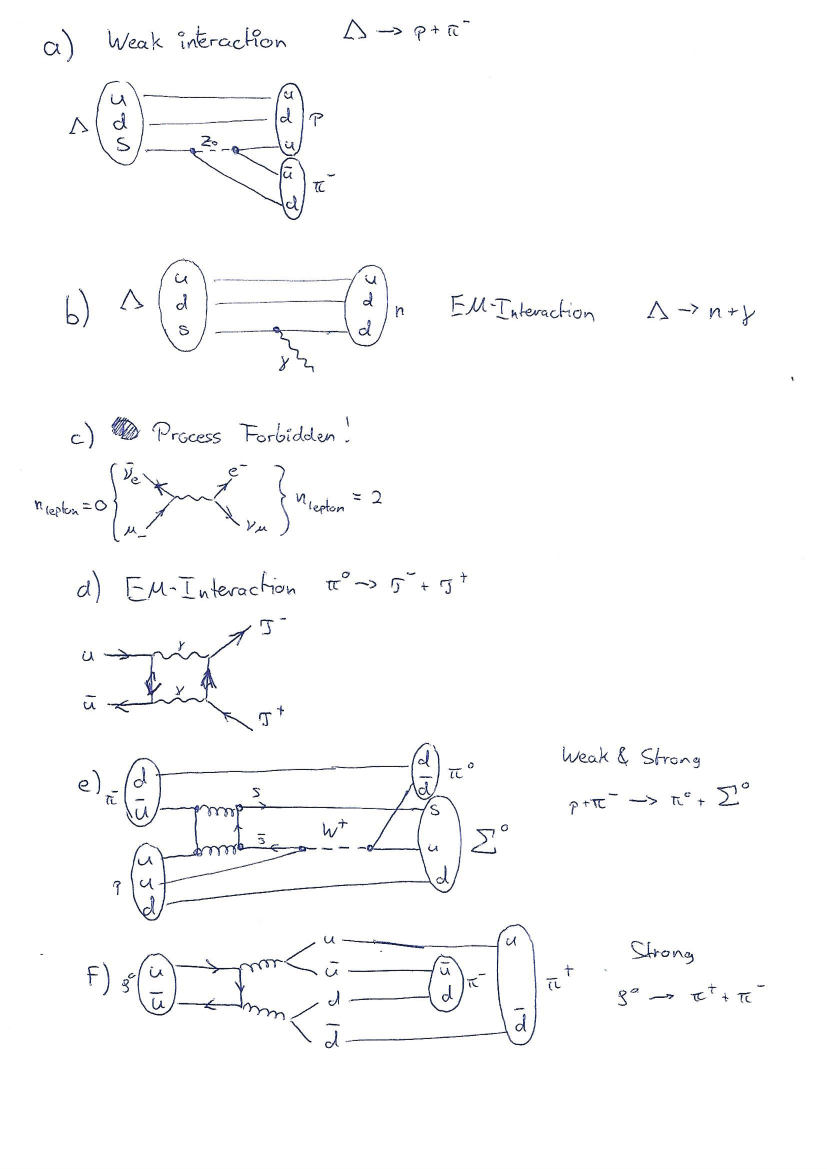
\includegraphics[trim=0 80 0 10,clip,width=\textwidth]{sheet_1_scan.png}
    \caption{Feynman Diagrams for the given processes}
    \label{figure:feynman}
\end{figure}
\end{document}
